% Campus Event Management System - Project Report
% Compile with: pdflatex report.tex (run twice for TOC/List of Figures)
% Optional images (place beside report.tex; if missing, a placeholder box is shown):
%   logo.png, fig3_1.png, fig3_2.png, fig4_1.png ... fig4_6.png, fig5_1.png ... fig5_12.png
\documentclass[12pt,a4paper]{report}

\usepackage[T1]{fontenc}
\usepackage{mathptmx}
\usepackage[a4paper,left=3.5cm,right=2.5cm,top=2.5cm,bottom=2.5cm]{geometry}
\usepackage{graphicx}
\usepackage{array,tabularx,longtable}
\usepackage{setspace}
\usepackage{titlesec}
\usepackage{tikz}
\usetikzlibrary{positioning,arrows.meta,shapes.geometric,fit}
\usepackage[hidelinks]{hyperref}
\usepackage{caption}
\usepackage{tocloft}

\setstretch{1.3}
\setlength{\parindent}{0pt}
\setlength{\parskip}{6pt}
\captionsetup{labelsep=space,font=normalsize}

% Chapter headings: "Chapter N" / Title, centred, bold
\titleformat{\chapter}[display]{\centering\bfseries\Large}{Chapter \thechapter}{10pt}{\Large}
\titlespacing*{\chapter}{0pt}{0pt}{20pt}
\titleformat{\section}{\bfseries\large}{\thesection}{1em}{}
\titleformat{\subsection}{\bfseries\normalsize}{\thesubsection}{1em}{}

% Figure placeholder helper: \figbox{file}{height}{caption text}{label}
\newcommand{\figbox}[4]{%
  \begin{figure}[htbp]\centering
  \IfFileExists{#1}{\includegraphics[width=0.9\textwidth,height=#2,keepaspectratio]{#1}}%
  {\fbox{\parbox[c][#2][c]{0.85\textwidth}{\centering [Insert figure: #3]}}}
  \caption{#3}\label{#4}
  \end{figure}}

\newcommand{\shot}[3]{% \shot{file}{caption}{label}
  \figbox{#1}{6cm}{#2}{#3}}

\begin{document}

%%%%%%%%%%%%%%%%%%%% TITLE PAGE %%%%%%%%%%%%%%%%%%%%
\pagenumbering{gobble}
\begin{center}
\singlespacing
Project Report on\\[10pt]
{\LARGE\bfseries Campus Event Management System}\\[10pt]
Submitted in partial fulfilment of the requirements of the degree of\\[12pt]
{\large BACHELOR OF ENGINEERING}\\[8pt]
In\\[8pt]
{\large INFORMATION TECHNOLOGY ENGINEERING}\\[8pt]
by\\[8pt]
{\bfseries Vedashri Chaudhari (233105)\\
Chirag Bhoir (243158)\\
Yash Baviskar (243155)\\
Swayam Jadhav (243162)}\\[10pt]
Under the guidance of\\[8pt]
{\bfseries Prof. Sneha Sankhe}\\[10pt]
\IfFileExists{logo.png}{\includegraphics[height=3cm]{logo.png}}{\fbox{\parbox[c][2.5cm][c]{3cm}{\centering [College logo]}}}\\[14pt]
{\Large\bfseries Department of Information Technology Engineering}\\[6pt]
{\large\bfseries Theem College of Engineering, Boisar}\\[6pt]
Boisar Chilhar Road, Boisar (E), Palghar\\[8pt]
{\large\bfseries University of Mumbai}\\
2026--27
\end{center}
\newpage

%%%%%%%%%%%%%%%%%%%% CERTIFICATE %%%%%%%%%%%%%%%%%%%%
\begin{center}{\large\bfseries CERTIFICATE}\end{center}
This is to certify that the ROSP mini project entitled ``Campus Event Management System'' is a bonafide work of ``Vedashri Chaudhari (233105), Chirag Bhoir (243158), Yash Baviskar (243155), Swayam Jadhav (243162)'' submitted to the University of Mumbai in partial fulfilment of the requirement for the award of the degree of ``Bachelor of Engineering in Information Technology Engineering'' during the academic year 2026--27.

\vspace{3cm}
\noindent
\begin{tabularx}{\textwidth}{XXX}
\textbf{Prof. Sneha Sankhe}\newline Guide & \textbf{Prof. Sneha Sankhe}\newline HOD IT & \textbf{Dr. Riyazoddin Siddiqui}\newline Principal
\end{tabularx}
\newpage

%%%%%%%%%%%%%%%%%%%% APPROVAL %%%%%%%%%%%%%%%%%%%%
\begin{center}{\large\bfseries ROSP Mini Project Report Approval}\end{center}
This ROSP mini project report entitled \textbf{Campus Event Management System} by Vedashri Chaudhari (233105), Chirag Bhoir (243158), Yash Baviskar (243155), Swayam Jadhav (243162) is approved for the degree of Bachelor of Engineering in Information Technology Engineering from University of Mumbai.

\vspace{3cm}
\noindent
\begin{tabularx}{\textwidth}{XX}
INTERNAL EXAMINER & EXTERNAL EXAMINER
\end{tabularx}

\vspace{2cm}
Date:\\
Place:
\newpage

%%%%%%%%%%%%%%%%%%%% DECLARATION %%%%%%%%%%%%%%%%%%%%
\begin{center}{\large\bfseries Declaration}\end{center}
We declare that this written submission represents our ideas in our own words and where others' ideas or words have been included, we have adequately cited and referenced the original sources. We also declare that We have adhered to all principles of academic honesty and integrity and have not misrepresented or fabricated or falsified any idea/data/fact/source in my submission. We understand that any violation of the above will be cause for disciplinary action by the Institute and can also evoke penal action from the sources which have thus not been properly cited or from whom proper permission has not been taken when needed.

\vspace{1.5cm}
\begin{flushright}
Vedashri Chaudhari (233105)\\
Chirag Bhoir (243158)\\
Yash Baviskar (243155)\\
Swayam Jadhav (243162)
\end{flushright}
\vspace{1cm}
Date:
\newpage

%%%%%%%%%%%%%%%%%%%% FRONT MATTER %%%%%%%%%%%%%%%%%%%%
\pagenumbering{roman}
\setcounter{page}{1}

\chapter*{Abstract}
The Campus Event Management System is a web-based application designed to help a college manage events and student participation digitally. In many institutions, event announcements, registrations, attendance and participation certificates are still handled through notices, paper forms, spreadsheets and messaging groups, which leads to duplicated effort, errors and poor visibility of records. The objective of this project is to provide a single, role-based platform that covers the complete event life cycle, from event creation to certificate issue.

The system defines three user roles. The Admin manages users, oversees events, monitors system activities and accesses reports. The Organizer/Faculty creates and manages events, submits them for approval where applicable, monitors registrations, manages attendance and issues participation certificates. The Student browses available events, registers for them, views registration details, receives notifications and, where these features are available, uses QR-based passes and views or downloads certificates.

The application is built using React.js with Vite for the frontend, Node.js and Express.js for the backend REST API, and MongoDB with Mongoose for data storage. Authentication and authorisation are handled using JSON Web Tokens (JWT) and bcryptjs password hashing, while the QRCode, PDFKit, Nodemailer and Multer libraries support QR passes, PDF certificates, email notifications and file uploads respectively, wherever these modules are implemented. The system is expected to reduce manual paperwork, improve the accuracy of registration and attendance records, and give students, faculty and administrators timely and transparent access to event information.
\newpage

\chapter*{Organization of the Report}
The organization of this report is as follows.

\textbf{Chapter 1: Introduction.} This chapter gives a brief introduction about ``Campus Event Management System'' and includes the overview, motivation, problem definition, aim and scope of the project.

\textbf{Chapter 2: Literature Survey.} This chapter is divided into two sections: the first presents the background of event management, online registration, attendance tracking and digital certificates, and the second presents a literature review with a comparative analysis of related work.

\textbf{Chapter 3: System Architecture.} This chapter provides the requirement analysis (hardware and software requirements), the system architecture based on React.js, Node.js, Express.js and MongoDB, and the proposed system, giving the information necessary to understand the implementation of the project.

\textbf{Chapter 4: System Design.} This chapter presents the Sequence, Use Case and Activity diagrams, the ER diagram and the Level 0 and Level 1 Data Flow Diagrams to understand the connectivity and flow of the various activities.

\textbf{Chapter 5: Result and Discussion.} This chapter describes the system screens and workflows for the Admin, Organizer/Faculty and Student roles. Screenshot placeholders are provided where actual screenshots from the final build are to be inserted.

\textbf{Chapter 6: Conclusion and Future Scope.} This chapter presents the conclusion drawn from the project and the areas in which the work can be extended in future.
\newpage

\renewcommand{\contentsname}{List of Contents}
\tableofcontents
\newpage
\listoffigures
\newpage
\listoftables
\newpage

\chapter*{Acronyms}
\addcontentsline{toc}{chapter}{Acronyms}
\begin{tabular}{@{}ll}
API: & Application Programming Interface\\
CPU: & Central Processing Unit\\
CRUD: & Create, Read, Update, Delete\\
CSS: & Cascading Style Sheets\\
DFD: & Data Flow Diagram\\
ER: & Entity Relationship\\
HTML: & HyperText Markup Language\\
HTTPS: & HyperText Transfer Protocol Secure\\
IDE: & Integrated Development Environment\\
JSON: & JavaScript Object Notation\\
JWT: & JSON Web Token\\
ODM: & Object Document Mapper\\
PDF: & Portable Document Format\\
QR: & Quick Response\\
RAM: & Random Access Memory\\
REST: & Representational State Transfer\\
SMTP: & Simple Mail Transfer Protocol\\
SPA: & Single-Page Application\\
SSD: & Solid State Drive\\
UI: & User Interface\\
UML: & Unified Modeling Language\\
\end{tabular}
\newpage

%%%%%%%%%%%%%%%%%%%% MAIN MATTER %%%%%%%%%%%%%%%%%%%%
\pagenumbering{arabic}
\setcounter{page}{1}

%-------------------- Chapter 1 --------------------
\chapter{Introduction}

\section{An Overview}
The Campus Event Management System is a web-based application developed to help a college organise events and manage student participation digitally. Colleges conduct many activities during an academic year, such as technical workshops, seminars, cultural programmes, sports meets and guest lectures. The system provides a single platform where these events can be created, published, registered for, attended and recognised through participation certificates.

The system is designed around three user roles. The Admin manages users, oversees events, monitors system activities and accesses reports. The Organizer/Faculty creates and manages events, submits them for approval where applicable, monitors registrations, manages attendance and issues participation certificates. The Student browses the available events, registers for them, views registration details, receives event-related notifications and, where these features are available, uses a QR-based pass and views or downloads certificates.

The application is developed using React.js with Vite for the frontend, Node.js and Express.js for the backend, and MongoDB with Mongoose as the database. User authentication is based on JSON Web Tokens (JWT) with bcryptjs for password hashing. Supporting libraries such as QRCode, PDFKit, Nodemailer and Multer are used for QR passes, PDF certificates, email notifications and file uploads in the modules where these functions are implemented.

\section{Motivation}
Event management in many colleges still depends on printed notices, paper registration forms, shared spreadsheets and messaging groups. These methods make it difficult for students to find out about upcoming events, for organizers to know how many students have registered, and for faculty to maintain reliable attendance records. Participation certificates are usually prepared manually after the event, which takes time and may lead to spelling mistakes, missing names or delays.

A centralized web-based system can remove most of this manual effort. Students can see all events in one place and register in a few steps, organizers can monitor registrations and attendance as they happen, and administrators can obtain summaries without collecting data from several sources. This need for a simple, reliable and transparent digital solution motivated the development of the Campus Event Management System.

\section{Problem Definition}
Managing college events through manual and scattered methods is time-consuming and error-prone. Event information is spread across notice boards and chat groups, registrations are collected through paper forms or separate online forms, attendance is marked on sheets that are difficult to consolidate, and certificates are prepared separately for each event. As a result, there is no single, reliable record of which students registered for and attended which events.

There is therefore a need for a centralized system in which organizers can create and manage events, students can register and receive a unique registration identifier, attendance can be recorded by QR-based or manual methods, certificates can be issued and verified, and administrators can oversee all activities with proper role-based access.

\section{Aim}
The aim of the Campus Event Management System is to develop a secure, web-based platform that allows a college to manage the complete life cycle of its events, from event creation and approval to student registration, attendance and participation certificates. The system aims to reduce manual paperwork, improve the accuracy of registration and attendance records, provide timely notifications to students, and give the Admin, Organizer/Faculty and Student roles access to the information they need through a simple and consistent interface.

\section{Scope}
The scope of the Campus Event Management System covers the digital management of events organised within a college. It includes user registration and login with role-based access for Admin, Organizer/Faculty and Student; creation, editing and display of event details such as title, description, date, venue and registration information; student registration for events with a unique registration identifier; attendance marking using QR-based or manual methods; generation and verification of participation certificates; event-related notifications; and registration and attendance summaries for reports.

The functions that depend on additional libraries, namely QR pass generation (QRCode), PDF certificate generation (PDFKit), email notifications (Nodemailer) and file uploads (Multer), form part of the intended design and are described in this report to the extent supported by the project. The system is intended for use within a single college, and features such as online payment and a native mobile application are listed under future scope.

%-------------------- Chapter 2 --------------------
\chapter{Literature Survey}

\section{Background}
Events such as workshops, seminars, technical competitions and cultural programmes are an important part of student life in a college. Traditionally, their organisation has depended on printed circulars, paper or form-based registration, signature sheets for attendance and manually prepared certificates. With the growth of web technologies, institutions have started to adopt event management systems that publish event details online, accept registrations electronically and keep participant records in a database.

Attendance tracking has also moved from paper sheets to digital methods. Quick Response (QR) codes, standardised in ISO/IEC 18004~\cite{iso18004}, allow a code issued at registration to be scanned at the venue, which speeds up check-in and reduces manual entry. Similarly, certificates generated by the system from stored participation records can reduce delays and errors compared with manually prepared certificates. Full-stack JavaScript technologies, namely React.js for the interface, Node.js and Express.js for the server and MongoDB for data storage, offer a convenient way to build such systems as a single web application with a role-based REST API secured by JSON Web Tokens~\cite{rfc7519}.

\section{Literature Review}

\subsection{Web-Based Event Management for University Events}
M. P. P. Zaw (2019) described a web-based Event Management System intended to manage the seminars and events of a university. Members can view upcoming and past seminars and register online. The system was implemented using J2EE (Java), the Struts framework and a MySQL database~\cite{zaw}. The work demonstrates the benefit of online registration, but its description centres on event listing and registration and does not address attendance tracking or certificate issue.

\subsection{College Event Management System}
S. Mehta et al. (2024) presented a College Event Management System as a preprint that aims to replace manual event handling in a college or university with a digital platform. The described features include event scheduling, participant registration and viewing of registered events, with organizers able to create, manage and promote events and attendees able to explore and register for them. The keyphrases indicate a Bootstrap, PHP and SQL implementation~\cite{mehta}. The abstract does not describe QR-based attendance or certificate generation.

\subsection{UNIMAS Event Hub}
K. A. B. Kushairi (2025) developed the UNIMAS Event Hub, a web-based system for managing campus events at Universiti Malaysia Sarawak. The work identifies manual practices such as Google Forms registration, physical ticket distribution and messaging-app communication as sources of inefficiency. The system offers digital ticket generation, online payment, real-time event updates and tools for attendance tracking and feedback~\cite{kushairi}. It is oriented towards ticketing and payment, and certificate generation and verification are not described in the available abstract.

\subsection{QR Code-Based Attendance Systems}
G. Ambaye, M. S. Anderson and Y. Yihun (2026) presented a QR code based automated attendance tracking system for classroom management in which students scan personalised QR codes that log their names, IDs and timestamps and produce Excel files~\cite{ambaye}. A. Abu Sneineh and W. A. Salah (2025) proposed a QR-code based attendance system for university students in which a camera acting as a QR reader and a PIC microcontroller scan student ID cards and compare the data with a database before storing the attendance record~\cite{sneineh}. Both works show that QR codes can speed up attendance recording, but they address classroom attendance rather than event registration, and the second depends on dedicated hardware.

\subsection{Digital Certificate Verification}
A. Rustemi et al. (2023) carried out a systematic literature review of blockchain-based systems for academic certificate verification. The review reports that blockchain can be used to issue unchangeable digital certificates and can make verification quicker, more reliable and independent of a central authority~\cite{rustemi}. Such approaches suit academic credentials but need additional infrastructure. For participation certificates in a single college, a simpler approach, in which the server stores each certificate with a unique identifier that can be checked against the database, is a practical alternative.

\section{Analysis Table}
\begin{longtable}{|p{0.7cm}|p{3.4cm}|p{2.6cm}|p{3.3cm}|p{3.3cm}|}
\caption{Analysis Table}\label{tab:analysis}\\
\hline \textbf{Sr. No.} & \textbf{Paper Title} & \textbf{Author Name} & \textbf{Advantages} & \textbf{Research Gap}\\ \hline
\endfirsthead
\hline \textbf{Sr. No.} & \textbf{Paper Title} & \textbf{Author Name} & \textbf{Advantages} & \textbf{Research Gap}\\ \hline
\endhead
1 & Web-Based Event Management System (EMS) & M. P. P. Zaw, 2019 & Online listing of university seminars and events with online registration. & Does not describe QR-based attendance, certificates or role-based approval; Java (J2EE/Struts) and MySQL based.\\ \hline
2 & College Event Management System & S. Mehta et al., 2024 & Event scheduling, participant registration and organizer tools to create and manage events. & Abstract does not describe QR attendance or certificate generation.\\ \hline
3 & UNIMAS Event Hub: A Web-Based System for Managing Campus Events & K. A. B. Kushairi, 2025 & Digital tickets, real-time updates, attendance tracking and feedback tools. & Oriented to ticketing and payment; certificate generation not described.\\ \hline
4 & Automated QR Code Attendance Tracking System for Efficient Classroom Management & G. Ambaye et al., 2026 & Fast QR-based attendance with logged names, IDs and timestamps; less paperwork. & Designed for classroom attendance; not linked to event registration or certificates.\\ \hline
5 & A Systematic Literature Review on Blockchain-Based Systems for Academic Certificate Verification & A. Rustemi et al., 2023 & Tamper-resistant and quicker verification of digital certificates. & Concerned with academic credentials; needs blockchain infrastructure; no event or attendance management.\\ \hline
\end{longtable}

%-------------------- Chapter 3 --------------------
\chapter{System Architecture}

\section{Introduction}
The Campus Event Management System is designed as a three-tier web application that provides a centralised and systematic approach for managing college events, student registrations, attendance and participation certificates. The system has separate interfaces and permissions for the Admin, Organizer/Faculty and Student roles. The React.js frontend communicates with a Node.js and Express.js REST API, which applies authentication and role-based authorisation and stores data in MongoDB through Mongoose. This chapter describes the requirements, the architecture and the proposed system.

\section{Design}

\subsection{Requirement Analysis}
The requirements of the Campus Event Management System are grouped into hardware requirements and software requirements.

\textbf{Hardware Requirements}

The system is a web application and does not need specialised hardware. A standard computer capable of running a modern browser, Node.js and MongoDB is sufficient for development and testing, while users can access the application from any device with a web browser and an Internet connection. For QR-based attendance, a device with a camera, such as a smartphone or a laptop, is required.

\begin{table}[htbp]
\centering
\caption{Hardware Requirements}\label{tab:hw}
\begin{tabular}{|p{4.5cm}|p{8cm}|}
\hline \textbf{Component} & \textbf{Specification / Description}\\ \hline
Personal Computer / Laptop & Used for development, deployment and testing of the system.\\ \hline
Processor & Intel Core i5 or higher (or equivalent).\\ \hline
RAM & Minimum 8 GB (16 GB preferred for running the frontend, backend and database together).\\ \hline
Storage & 256 GB SSD or higher (for project files, the database and uploaded files).\\ \hline
Camera & Webcam or smartphone camera for scanning QR passes during attendance (where QR attendance is used).\\ \hline
Internet Connectivity & Required for accessing the web application, sending email notifications and installing packages.\\ \hline
\end{tabular}
\end{table}

\textbf{Software Requirements}

The software stack of the Campus Event Management System combines a React.js frontend, a Node.js and Express.js backend and a MongoDB database. Authentication is based on JWT and bcryptjs, and additional libraries support QR passes, PDF certificates, email notifications and file uploads where these modules are implemented~\cite{react}--\cite{nodejs}.

\begin{table}[htbp]
\centering
\caption{Software Requirements}\label{tab:sw}
\begin{tabular}{|p{4.5cm}|p{8cm}|}
\hline \textbf{Category} & \textbf{Specification / Tools Used}\\ \hline
Operating System & Windows 10/11, Linux (Ubuntu 20.04 or later) or macOS.\\ \hline
Frontend & React.js with Vite.\\ \hline
Backend & Node.js and Express.js (REST API).\\ \hline
Database & MongoDB with Mongoose (ODM).\\ \hline
Authentication & JSON Web Token (JWT) and bcryptjs.\\ \hline
Supporting Libraries & QRCode (QR passes), PDFKit (PDF certificates), Nodemailer (email notifications), Multer (file uploads), where implemented.\\ \hline
Development Tools & Visual Studio Code and a modern web browser.\\ \hline
\end{tabular}
\end{table}

\subsection{System Architecture}
The system follows a three-tier architecture, shown in Fig.~\ref{fig:arch}. Users access the application through a web browser. The presentation layer is a React.js single-page application built with Vite. It sends REST API requests in JSON format to the application layer, which is implemented with Node.js and Express.js. Middleware verifies the JWT and the role of the user before a request reaches the Auth, Event, Registration, Attendance, Certificate and Notification and Report modules. These modules use Mongoose schemas and models to store and retrieve data from MongoDB, and use the QRCode, PDFKit, Nodemailer and Multer libraries where the corresponding functions are implemented.

\begin{figure}[htbp]
\centering
\IfFileExists{fig3_1.png}{\includegraphics[width=0.95\textwidth]{fig3_1.png}}{%
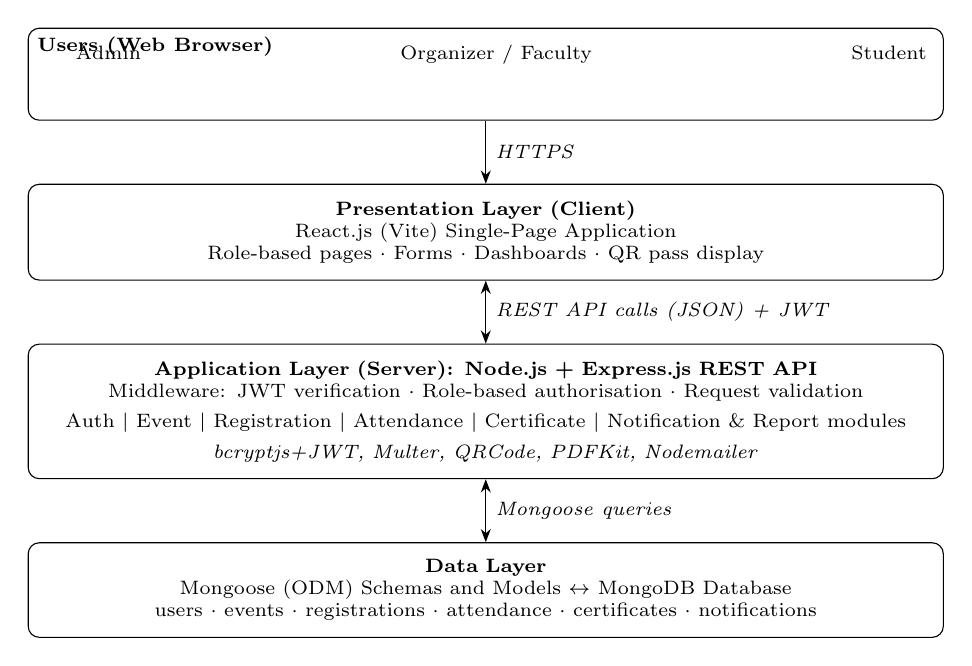
\begin{tikzpicture}[font=\scriptsize,box/.style={draw,rounded corners,align=center,minimum height=0.7cm,inner sep=3pt},
 layer/.style={draw,rounded corners,inner sep=6pt,text width=11.2cm},>=Stealth]
\node[layer,label={[anchor=north west,font=\scriptsize\bfseries]north west:Users (Web Browser)}] (u) {\vspace{0.5cm}\hspace{0.3cm} Admin \hfill Organizer / Faculty \hfill Student\hspace{0.3cm}};
\node[layer,below=0.8cm of u,align=center] (p) {\textbf{Presentation Layer (Client)}\\ React.js (Vite) Single-Page Application\\ Role-based pages $\cdot$ Forms $\cdot$ Dashboards $\cdot$ QR pass display};
\node[layer,below=0.8cm of p,align=center] (a) {\textbf{Application Layer (Server): Node.js + Express.js REST API}\\ Middleware: JWT verification $\cdot$ Role-based authorisation $\cdot$ Request validation\\[3pt]
Auth $\mid$ Event $\mid$ Registration $\mid$ Attendance $\mid$ Certificate $\mid$ Notification \& Report modules\\[3pt]
\emph{bcryptjs+JWT, Multer, QRCode, PDFKit, Nodemailer}};
\node[layer,below=0.8cm of a,align=center] (d) {\textbf{Data Layer}\\ Mongoose (ODM) Schemas and Models $\leftrightarrow$ MongoDB Database\\ users $\cdot$ events $\cdot$ registrations $\cdot$ attendance $\cdot$ certificates $\cdot$ notifications};
\draw[->] (u) -- node[right]{\emph{HTTPS}} (p);
\draw[<->] (p) -- node[right]{\emph{REST API calls (JSON) + JWT}} (a);
\draw[<->] (a) -- node[right]{\emph{Mongoose queries}} (d);
\end{tikzpicture}}
\caption{System Architecture}\label{fig:arch}
\end{figure}

\subsection{Proposed System}
The proposed system is a role-based, web-based solution that digitises the complete event life cycle of a college. It provides three panels for the different user roles:

\begin{itemize}
\item \textbf{Admin Panel:} Allows the admin to manage users, oversee events, monitor system activities and access reports.
\item \textbf{Organizer/Faculty Panel:} Enables organizers to create and manage events, submit events for approval where applicable, monitor registrations, manage attendance and issue participation certificates.
\item \textbf{Student Panel:} Allows students to browse events, register for them, view registration details, receive notifications and access QR-based passes and certificates where implemented.
\end{itemize}

The main functional modules are Event Management, Registration Management, Attendance Management, Certificate Management, and Notifications and Reports. The proposed system replaces paper forms, spreadsheets and scattered messages with a single platform. Event data, registrations, attendance and certificate records are stored in MongoDB, and every request to the REST API is authenticated with a JWT and checked against the role of the user.

The QR pass, PDF certificate, email notification and file upload functions are provided through the QRCode, PDFKit, Nodemailer and Multer libraries respectively. They are described here as part of the intended design, and their availability depends on the final implementation of the project.

\begin{figure}[htbp]
\centering
\IfFileExists{fig3_2.png}{\includegraphics[width=0.95\textwidth]{fig3_2.png}}{%
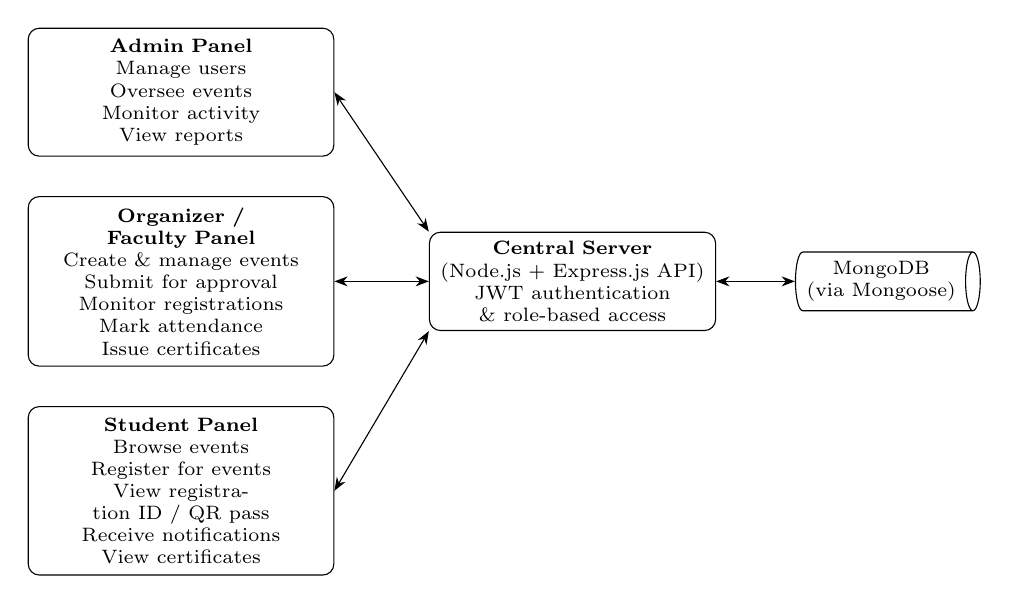
\begin{tikzpicture}[font=\scriptsize,node distance=0.8cm,
 pnl/.style={draw,rounded corners,align=center,text width=3.6cm,inner sep=4pt},>=Stealth]
\node[pnl] (ad) {\textbf{Admin Panel}\\Manage users\\Oversee events\\Monitor activity\\View reports};
\node[pnl,below=0.5cm of ad] (og) {\textbf{Organizer / Faculty Panel}\\Create \& manage events\\Submit for approval\\Monitor registrations\\Mark attendance\\Issue certificates};
\node[pnl,below=0.5cm of og] (st) {\textbf{Student Panel}\\Browse events\\Register for events\\View registration ID / QR pass\\Receive notifications\\View certificates};
\node[draw,rounded corners,align=center,text width=3.4cm,right=1.2cm of og] (sv) {\textbf{Central Server}\\(Node.js + Express.js API)\\JWT authentication \& role-based access};
\node[draw,cylinder,shape aspect=0.25,align=center,right=1cm of sv] (db) {MongoDB\\(via Mongoose)};
\draw[<->] (ad.east) -- (sv.north west);
\draw[<->] (og) -- (sv);
\draw[<->] (st.east) -- (sv.south west);
\draw[<->] (sv) -- (db);
\end{tikzpicture}}
\caption{Proposed System}\label{fig:proposed}
\end{figure}

%-------------------- Chapter 4 --------------------
\chapter{System Design}

\section{Introduction}
The Campus Event Management System is designed as a centralised web-based system for managing college events, student registrations, attendance and participation certificates. This chapter presents the design of the system using UML diagrams, an Entity Relationship (ER) diagram and Data Flow Diagrams (DFD). The system follows a client--server architecture in which the React.js frontend (built with Vite) communicates with a Node.js and Express.js REST API. The API handles authentication, authorisation and business logic, and stores data in MongoDB through Mongoose. The diagrams show the intended design of the system and the way data and control flow between users, the application and the database.

\section{UML Diagrams}
The Unified Modeling Language (UML) is a standardised approach used to visualise the design of a system. It helps in understanding system behaviour, relationships between modules and the overall flow of control. In this section the Sequence, Use Case and Activity diagrams are presented for the Campus Event Management System.

\subsection{Sequence Diagram}
The Sequence Diagram depicts the interaction between the system components over time. Fig.~\ref{fig:seq} shows the messages exchanged between the Student, Organizer/Faculty, React.js frontend, Express.js API server and MongoDB for login, event registration, attendance marking and certificate issue.

\figbox{fig4_1.png}{14cm}{Sequence Diagram}{fig:seq}

\subsection{Use Case Diagram}
The Use Case Diagram illustrates the interactions between the users (actors) and the system. Fig.~\ref{fig:usecase} shows how the Student, Organizer/Faculty and Admin interact with the application to perform their respective tasks.

\figbox{fig4_2.png}{10cm}{Use Case Diagram}{fig:usecase}

\subsection{Activity Diagram}
The Activity Diagram describes the flow of activities in the system, showing how users perform operations step by step. Fig.~\ref{fig:activity} shows the flow from login, through event creation and approval, to student registration, attendance marking and certificate issue.

\figbox{fig4_3.png}{12cm}{Activity Diagram}{fig:activity}

\subsection{ER Diagram}
The Entity Relationship (ER) Diagram defines the logical structure of the database used in the Campus Event Management System. It identifies the entities, their attributes and the relationships between them. The entities are User, Event, Registration, Attendance, Certificate and Notification, which are stored as MongoDB collections and related through ObjectId references defined using Mongoose schemas. The attributes shown in Fig.~\ref{fig:er} are the proposed fields of the data model.

\figbox{fig4_4.png}{9cm}{ER Diagram}{fig:er}

\section{Data Flow Diagram (DFD)}
The Data Flow Diagram (DFD) represents the flow of information within the system. It helps to understand how data is input, processed and output between the various processes, data stores and external entities.

\subsection{Level 0 DFD}
The Level 0 DFD (also called the context diagram) provides a high-level overview of the system. It shows the system as a single process and its interactions with the external entities Admin, Organizer/Faculty and Student.

\figbox{fig4_5.png}{7cm}{Level 0 Data Flow Diagram}{fig:dfd0}

\subsection{Level 1 DFD}
The Level 1 DFD breaks the main process into six sub-processes: authentication and user management, event management, registration management, attendance management, certificate management, and notifications and reports. It also shows the data stores used by these processes (users, events, registrations, attendance, certificates and notifications) and how data moves between them.

\figbox{fig4_6.png}{12cm}{Level 1 Data Flow Diagram}{fig:dfd1}

%-------------------- Chapter 5 --------------------
\chapter{Result and Discussion}
This chapter describes the screens and workflows of the Campus Event Management System for the Admin, Organizer/Faculty and Student roles. The descriptions explain what each screen is designed to provide. Where an actual screenshot from the final build is not yet available, a clearly labelled placeholder is given, to be replaced with the real screenshot; no screen in this chapter should be read as a result of testing or deployment unless a real screenshot is inserted. Features that depend on additional libraries, such as the QR pass, certificates and email notifications, are described to the extent that they are implemented in the final system.

\section{Home Page}
The home page is designed as the landing page of the system. It introduces the Campus Event Management System, shows upcoming events and provides links to login and registration. [A screenshot of the actual Home Page is to be inserted below.]
\shot{fig5_1.png}{Home Page}{fig:home}

\section{Login and Registration}
Users register with their details and log in with their credentials. Passwords are stored as bcryptjs hashes, and a JWT is issued on successful login. After login, the user is taken to the dashboard that matches the assigned role. [A screenshot of the actual Login and Registration is to be inserted below.]
\shot{fig5_2.png}{Login and Registration}{fig:login}

\section{Admin Dashboard}
The Admin Dashboard gives the admin access to user management, an overview of all events, monitoring of system activities and reports. [A screenshot of the actual Admin Dashboard is to be inserted below.]
\shot{fig5_3.png}{Admin Dashboard}{fig:admin}

\section{Organizer/Faculty Dashboard}
The Organizer/Faculty Dashboard lists the events created by the organizer and provides access to event creation, registration lists, attendance and certificate issue. [A screenshot of the actual Organizer/Faculty Dashboard is to be inserted below.]
\shot{fig5_4.png}{Organizer/Faculty Dashboard}{fig:org}

\section{Student Dashboard}
The Student Dashboard shows the events available to the student, the events the student has registered for, notifications and certificates. [A screenshot of the actual Student Dashboard is to be inserted below.]
\shot{fig5_5.png}{Student Dashboard}{fig:stud}

\section{Event Creation and Management}
Organizers create an event by entering its title, description, date, time, venue and registration details. Existing events can be edited, and events are submitted for approval where the approval step is applicable. [A screenshot of the actual Event Creation and Management is to be inserted below.]
\shot{fig5_6.png}{Event Creation and Management}{fig:evcreate}

\section{Event Browsing and Details}
Students browse the list of available events and open an event to view its description, date, venue and registration information. [A screenshot of the actual Event Browsing and Details is to be inserted below.]
\shot{fig5_7.png}{Event Browsing and Details}{fig:evbrowse}

\section{Event Registration and Registration ID}
A student registers for an event from its details page. Each registration is stored with a unique registration identifier, and duplicate registration for the same event is prevented. [A screenshot of the actual Event Registration and Registration ID is to be inserted below.]
\shot{fig5_8.png}{Event Registration and ID}{fig:evreg}

\section{QR Pass}
Where QR passes are implemented, a QR code generated with the QRCode library is shown for each registration and is used to identify the student at the venue. [A screenshot of the actual QR Pass is to be inserted below.]
\shot{fig5_9.png}{QR Pass}{fig:qr}

\section{Attendance Management}
Organizers mark attendance by scanning the QR pass or by selecting students manually, depending on the implemented functionality. The attendance records are stored against the registrations. [A screenshot of the actual Attendance Management is to be inserted below.]
\shot{fig5_10.png}{Attendance Management}{fig:att}

\section{Certificate Generation and Verification}
Where implemented, participation certificates are generated as PDF files with PDFKit for students whose attendance is recorded. Each certificate carries a unique identifier that can be used for verification. [A screenshot of the actual Certificate Generation and Verification is to be inserted below.]
\shot{fig5_11.png}{Certificate Generation and Verification}{fig:cert}

\section{Notifications and Reports}
Event-related notifications inform students about registration and event updates, and may be sent by email using Nodemailer where implemented. Reports summarise registrations and attendance for organizers and the admin. [A screenshot of the actual Notifications and Reports is to be inserted below.]
\shot{fig5_12.png}{Notifications and Reports}{fig:notif}

%-------------------- Chapter 6 --------------------
\chapter{Conclusion and Future Scope}

\section{Conclusion}
The Campus Event Management System provides a centralised, web-based platform for managing college events and student participation. It brings event creation, publication, registration, attendance and participation certificates into a single role-based application with separate interfaces for the Admin, Organizer/Faculty and Student. The use of React.js with Vite, Node.js with Express.js, and MongoDB with Mongoose gives the system a consistent JavaScript-based technology stack, while JWT and bcryptjs provide authentication and password protection.

The design reduces dependence on paper forms, spreadsheets and messaging groups, and is expected to improve the accuracy of registration and attendance records, make event information easier to find, and shorten the time taken to prepare participation certificates. The QR pass, PDF certificate, email notification and file upload functions, supported by the QRCode, PDFKit, Nodemailer and Multer libraries, form part of the intended design and are included to the extent implemented in the final system. Testing results and user feedback are not included in this report and can be added after evaluation of the completed system.

\section{Future Scope}
The system can be extended in several ways. A mobile application or progressive web app can make QR check-in and notifications more convenient. Event feedback forms and analytics dashboards can help organizers evaluate events, while online payment can support paid workshops. Additional notification channels such as SMS or push notifications, calendar integration, and integration with the college's student information system can further reduce manual work. For certificates, digital signatures or tamper-evident verification can be added, and the system can be deployed across multiple departments or institutions with additional access-control rules and performance monitoring.

%-------------------- References --------------------
\begin{thebibliography}{99}
\addcontentsline{toc}{chapter}{References}
\renewcommand{\bibname}{References}
\bibitem{zaw} M. P. P. Zaw, ``Web-Based Event Management System (EMS),'' \emph{Int. J. Trend in Scientific Research and Development (IJTSRD)}, vol. 3, no. 4, pp. 1640--1643, Jun. 2019, doi: 10.31142/ijtsrd25209.
\bibitem{mehta} S. Mehta, K. S. Goud, K. Pavankalyan, J. K. Kumar, and D. Srinivas, ``College Event Management System,'' EasyChair Preprint 12826, Mar. 2024. [Online]. Available: \url{https://easychair.org/publications/preprint/nmHZ}
\bibitem{kushairi} K. A. B. Kushairi, ``UNIMAS Event Hub: A Web-Based System for Managing Campus Events,'' Universiti Malaysia Sarawak, 2025. [Online]. Available: \url{https://scholarhub.unimas.my/handle/123456789/347}
\bibitem{ambaye} G. Ambaye, M. S. Anderson, and Y. Yihun, ``Automated QR Code Attendance Tracking System for Efficient Classroom Management,'' in \emph{Proc. 2026 ASEE Annual Conference \& Exposition}, Paper ID 53751. [Online]. Available: \url{https://nemo.asee.org/public/conferences/374/papers/53751/view}
\bibitem{sneineh} A. Abu Sneineh and W. A. Salah, ``Smart Attendance System for University Students Based on QR Code,'' \emph{Journal of Electrical and Electronics Engineering}, vol. 18, no. 1, pp. 5--10, May 2025. [Online]. Available: \url{https://doaj.org/article/ec02c8f32454498283a8fc54d5efe74f}
\bibitem{rustemi} A. Rustemi, F. Dalipi, V. Atanasovski, and A. Risteski, ``A Systematic Literature Review on Blockchain-Based Systems for Academic Certificate Verification,'' \emph{IEEE Access}, vol. 11, pp. 64679--64696, 2023, doi: 10.1109/ACCESS.2023.3289598.
\bibitem{rfc7519} M. Jones, J. Bradley, and N. Sakimura, ``JSON Web Token (JWT),'' RFC 7519, Internet Engineering Task Force, May 2015. [Online]. Available: \url{https://www.rfc-editor.org/info/rfc7519}
\bibitem{provos} N. Provos and D. Mazi\`eres, ``A Future-Adaptable Password Scheme,'' in \emph{Proc. USENIX Annual Technical Conference (FREENIX Track)}, 1999, pp. 81--91.
\bibitem{iso18004} ISO/IEC 18004:2015, \emph{Information technology --- Automatic identification and data capture techniques --- QR Code bar code symbology specification}, International Organization for Standardization, 2015.
\bibitem{react} React Documentation. [Online]. Available: \url{https://react.dev}
\bibitem{express} Express.js Documentation. [Online]. Available: \url{https://expressjs.com}
\bibitem{mongodb} MongoDB Documentation. [Online]. Available: \url{https://www.mongodb.com/docs/}
\bibitem{mongoose} Mongoose Documentation. [Online]. Available: \url{https://mongoosejs.com/docs/}
\bibitem{vite} Vite Documentation. [Online]. Available: \url{https://vite.dev/guide/}
\bibitem{nodejs} Node.js Documentation. [Online]. Available: \url{https://nodejs.org/en/docs}
\end{thebibliography}
\newpage

%-------------------- Acknowledgement --------------------
\chapter*{Acknowledgement}
\addcontentsline{toc}{chapter}{Acknowledgement}
We would like to take this opportunity to express our gratitude towards all the people who have in various ways helped in the successful completion of our project.

We must convey our gratitude to our honorable director Dr. N. K. Rana for being a constant source of inspiration throughout the project. We extend our gratitude to our respected Principal Dr. Riyazoddin Siddiqui and our HOD and Project Guide Prof. Sneha Sankhe for their invaluable guidance, support and help in preparing the project, personally correcting our work and providing encouragement throughout the project. Additionally, we extend our appreciation to all the teaching staff, whose profound knowledge, passion for teaching and dedication to students' learning have been a constant source of inspiration and motivation. We are also thankful to all the non-teaching staff for their behind-the-scenes efforts in maintaining the infrastructure, administrative support and logistical assistance that contributed to the project's success. We would also like to thank our parents, whose unwavering love, encouragement and sacrifices have been the cornerstone of our journey. Their belief in our abilities and endless support have been a constant source of strength and motivation. Finally, we are grateful to our family and friends for their understanding, encouragement and unwavering support throughout this endeavour.

We also thank all our faculty members for steering us through the tough as well as easy phases of the project in a result-oriented manner with concerned attention.

\vspace{1cm}
\begin{flushright}
Vedashri Chaudhari (233105)\\
Chirag Bhoir (243158)\\
Yash Baviskar (243155)\\
Swayam Jadhav (243162)
\end{flushright}

\end{document}
